\section{Klasser}
\label{klasser}
En HiFi-forstærkers udgangstrin kan designes på forskellige måder alt efter hvilke karakteristika man ønsker at opnå. De forskellige designs er opdelt i klasser. Klasserne er bestemt ud fra en karakteristik og ikke ud fra en bestemt opkobling af kredsløbet. 
I dette afsnit vil der blive gjort rede for de gængse klassifikationer, som har med analogt opbyggede forstærkere at gøre, og forklare hvilke fordele og ulemper der er med dem. Redegørelsen vil tage udgangspunkt i et eksempel på et kredsløb, som har den pågældende klasses karakteristika. 
Der vil, på baggrund af dette afsnit, blive valgt en endelig udgangstrinsklasse til dette projekts HiFi-forstærker hvilket vil blive, et krav i kravspecifikationen.

\subsection{Klasse A}

Et klasse A udgangstrin har en collectorstrøm, som vist på figur \ref{fig:klassea} med en sinustone, som indgangssignal. 

\begin{figure}[h]
\centering
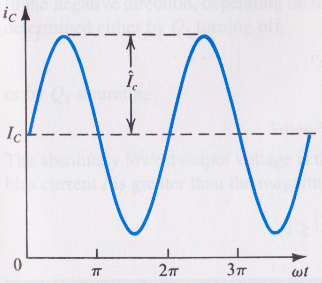
\includegraphics[scale=.35]{indledende_analyse/klasser/klassea.png}
\caption{Klasse A $i_c$ karakteristik}
\label{fig:klassea}
\end{figure}

Et klasse A trins udgangsstrøm er centreret om en DC-strøm, hvilket betyder at der, i modsætning til klasse B, afsættes effekt i trinnet i hviletilstand. Dette gør at den maksimale virkningsgrad kun er 25\%. Dog er et klasse A trin det mest transparente, altså det med mindst forvrængning.

Et klasse A udgangstrin kan opbygges af to NPN transistorer, Q1 og Q2, i en emitterfølgerkobling, som vist på figur \ref{fig:classa}. En konstant strøm løber gennem Q2, da $v_{BE2}$ er konstant. Inputsignalet kommer ind på Q1's base og styrer således strømmen der kan løbe gennem Q1 og loadmodstanden. 

\begin{figure}[h]
\centering
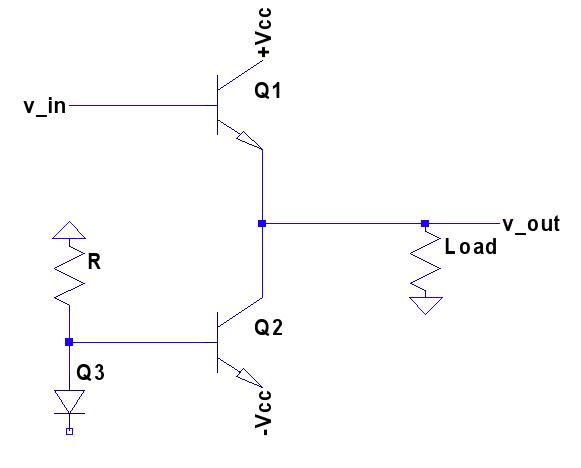
\includegraphics[scale=.35]{indledende_analyse/klasser/classa.png}
\caption{Klasse A forstærker kredsløb}
\label{fig:classa}
\end{figure}

Et klasse A trin er et godt trin forvrængningsmæssigt, men virkningsgraden er, sammenlignet med de andre trin, meget lille, hvilket også er en af grundene til at det sjældent bruges i moderne HiFi-forstærkere.

\subsection{Klasse B}

Et klasse B udgangstrin har en collectorstrøm, som vist på figur \ref{fig:klasseb} med en sinustone, som indgangssignal. 

\begin{figure}[h]
\centering
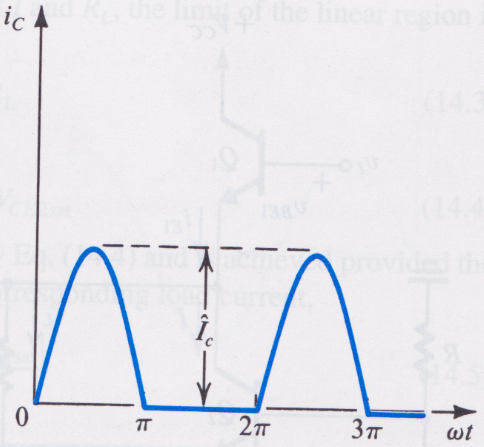
\includegraphics[scale=.35]{indledende_analyse/klasser/klasseb.png}
\caption{Klasse B $i_c$ karakteristik}
\label{fig:klasseb}
\end{figure}

Et klasse B trin overfører kun en halv periode af indgangssignalet til udgangen. For at kunne gengive et udgangssignal similært til indgangssignalet er det derfor nødvendigt at sammensætte to klasse B trin således at det ene tager sig af den positive halvperiode og den anden den negative.
Et klasse B trin har en maksimal nyttevirkning på 50\%.

I nedenstående eksempel er klasse B trinnet opbygget af to transistorer, en NPN (Q1) og en PNP (Q2), som vist på figur \ref{fig:classb}. Når input spændingen overstiger ca. 0,5 V vil Q1 begynde at lede strøm til loadmodstanden mens Q2 er lukket. Kommer input spændingen under -0,5 V vil Q2 lede, men da Q2 er en PNP vil den trække strøm mod -Vcc hvormed der trækkes strøm fra loadmodstanden. Når Q2 leder er Q1 lukket. 

\begin{figure}[h]
\centering
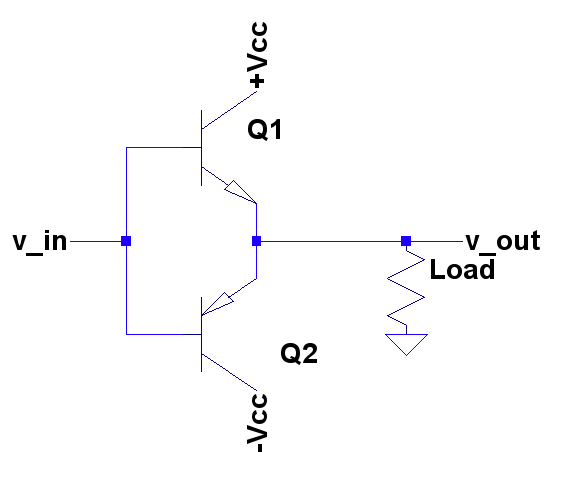
\includegraphics[scale=.35]{indledende_analyse/klasser/classb.png}
\caption{Klasse B forstærker kredsløb}
\label{fig:classb}
\end{figure}

\subsection{Klasse AB}

Et klasse AB udgangstrin har en collectorstrøm, som vist på figur \ref{fig:klasseab} med en sinustone, som indgangssignal. 

\begin{figure}[h]
\centering
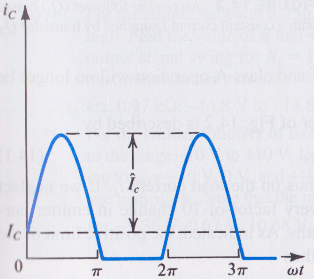
\includegraphics[scale=.35]{indledende_analyse/klasser/klasseab.png}
\caption{Klasse AB $i_c$ karakteristik}
\label{fig:klasseab}
\end{figure}

Dette trin overfører lidt mere end en halv periode af indgangssignalet til udgangen. Dette bevirker at, hvis man bruger samme teknik, som ved et klasse B trin til at få en hel sinusperiode på udgangen, vil de to signaler overlappe i overgangsperioden. Dette medvirker til at crossover-forvrængningen, som klasse B havde tendenser til, elemineres. 
Et klasse AB trin har en maksimal nyttevirkning på 75\%.

Der tages i følgende eksempel på et klasse AB trin udgangspunkt i klasse B trinnet på figur \ref{eq:classb}, med den forskel at potentialet på Q1 og Q2's base er hævet til saturationspændingen når signalspændningen er 0 V. Det er denne forskel, som eleminerer crossover forvrængningen.
Klasse AB er det oftest benyttede i moderne HiFi-forstærkere fordi det har lav forvrængning, høj nyttevirkning og er relativt let at få et godt resultat ud af. \fixme{ref til sedra/smith}

\begin{figure}[h]
\centering
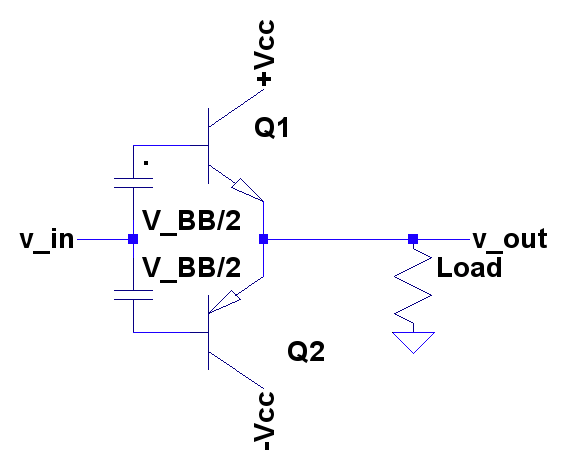
\includegraphics[scale=.35]{indledende_analyse/klasser/classab.png}
\caption{Klasse AB forstærker kredsløb}
\label{fig:classab}
\end{figure}


\subsection{Delkonklusion}


\fixme{skriv om virkningsgrad i stedet for at snakke løst om effektforbrug}
\fixme{indsæt grafer som viser outputtet af de forskellige}
